The results visualization system provides a graphical summary of the progression of an optimziation. It was written using Ruby On Rails and takes advantage of two graphical plotting tools: gcharts and graphviz. Gcharts is used to generate the graphcial plots of relevant optimization metrics from different optimizations. The graphviz package is used to render images of the 

\subsection{Optimization Metrics}
The progress of the optimziation is charachertized on a per generation bassis. Relevant metrics include: 
\begin{itemize}
	\item Average fitness
	\item Maximum fitness
	\item Std. deviation of fitness
\end{itemize}

For a good optimization one would expect both the maximum fitness and the average fitness to increase from one generation to the next. However, for this optimization it is also important that population diversity is maintained as well. Both the competition and the mutation parameters were selected to maintain population diversity. The Std. deviation, $\sigma$, of the population gives an indication of the diversity of the population in any given generation. 

\subsection{TM Representation}
The vizualization of individual TMs provides a valuable tool for their inspection. There are litterally thousands of TMs created over the course of an optimziation, and graphviz package allows or the creation of a state transition diagram for quick visual inspection of particular TMs. Figure \ref{fig:example_TM} is the state transition diagram for the example TM in Table \ref{tab:example_TM}. This visual representation is much easier to interperate than the state transition table. 

\begin{figure}[!hbp]
	\centering 
	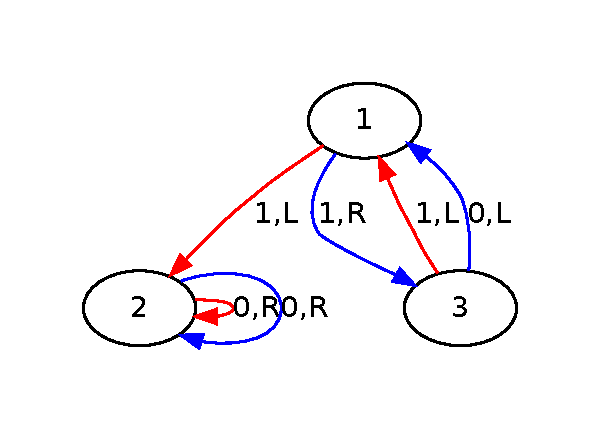
\includegraphics[width=.8\textwidth]{images/example_TM}
	\caption{State transition diagram for notional 3-state TM. Edge color indicates the bit being read from the tape (red=0,blue=1). Edge label indicates the write bit and movement direction for a given transition.}
	\label{fig:example_TM}
\end{figure}
